\documentclass{article}
\usepackage[utf8]{inputenc}
\usepackage{listings}
\usepackage{graphicx}
\usepackage{color}
\usepackage{amsmath}


\newcommand{\gromet}{GroMEt}
\newcommand{\smtlib}{SMTLib}
\newcommand{\gromettosmtlib}{\gromet2\smtlib}
\newcommand{\sn}{\gromettosmtlib}

\author{Dan Bryce\\dbryce@sift.net\\SIFT, LLC.}
\title{\sn~ Encoding Examples}

\begin{document}
\lstset {
    language=Python,
    frame=htb,
    tabsize=4,
    % showstringspaces=false,
    % numbers=left,
    % %upquote=true,
    % firstnumber=1,
    % stepnumber=1,
    % commentstyle=\color{commentgreen},
    % keywordstyle=\color{eminence},
    % stringstyle=\color{red},
    % basicstyle=\small\ttfamily, % basic font setting
    % emph={int,char,double,float,unsigned,void,bool},
    % emphstyle={\color{blue}},
    % escapechar=\&,
    % % keyword highlighting
    % classoffset=1, % starting new class
    % otherkeywords={>,<,.,;,-,!,=,~},
    % morekeywords={>,<,.,;,-,!,=,~},
    % keywordstyle=\color{weborange},
    % classoffset=0,
    numberstyle=\color{blue}, % the style that is used for the line-numbers
    breaklines=true,
    numbers=left, 
    frame=single, 
}

\maketitle

\section{Direct Encoding}

\begin{align}
    F.fn.x &= F.fn.pof[i] & :& \forall i \in range(|F.fn.pof|), x = F.fn.pof[i].name\\
    F.fn.pof[j] &= F.fn.bf[i].value.fn.opo[j']  & :& \forall i \in range(|F.fn.bf|), \notag \\
    &&& \forall j \in range(|F.fn.pof|) \;\text{where}\; F.fn.pof[j].box-1 = i,\notag \\
    &&& j' \in range(F.fn.bf[i].value.fn.opo),\\
    F.fn.opo[i] &= F.fn.pof[j] &:& \forall k \in range(F.fn.wfopo)\;\text{where} \notag \\ 
    &&&i = F.fn.wfopo[k].src-1,\notag\\
    &&& j = F.fn.wfopo[k].tgt-1\\
    F.fn.pif[i] &= F.fn.pof[j] &:& \forall k \in range(F.fn.wff)\;\text{where} \notag \\ 
    &&&i = F.fn.wfopo[k].src-1,\notag\\
    &&& j = F.fn.wfopo[k].tgt-1\\
\end{align}

\subsection{Examples}

\subsubsection{exp0}

\begin{lstlisting}[caption=Python code for example exp0., label=exp0]
x = 2
\end{lstlisting}



\begin{figure}[htb]
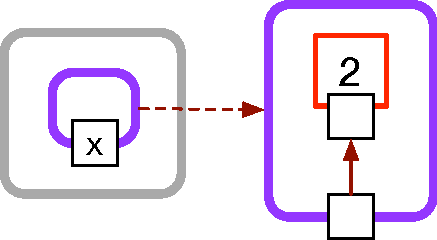
\includegraphics[width=0.5\linewidth]{fig/exp0_gromet_FN_manual_diagram.pdf}
\caption{\gromet Function network for exp0.}
\end{figure}


\lstinputlisting[caption=\gromet\ for example exp0., label=exp0]{gromet/exp0--Gromet-FN-auto.json}    

%(('exp0.fn.bf[0].value.fn.bf[0].value' = 2) & ('exp0.fn.bf[0].value.fn.pof[0]' = 'exp0.fn.bf[0].value.fn.bf[0].value') & ('exp0.fn.bf[0].value.fn.opo[0]' = 'exp0.fn.bf[0].value.fn.pof[0]') & ('exp0.fn.pof[0]' = 'exp0.fn.bf[0].value.fn.opo[0]') & (exp0.fn.x = 'exp0.fn.pof[0]'))

The following equations encode the semantics of the \gromet\ in Listing \ref{exp0}.
\begin{eqnarray*}
    exp0.fn.x &=& exp0.fn.pof[0]\\
    exp0.fn.pof[0] &=& exp0.fn.bf[0].value.fn.opo[0]\\
    exp0.fn.bf[0].value.fn.opo[0] &=& exp0.fn.bf[0].value.fn.pof[0]\\
    exp0.fn.bf[0].value.fn.pof[0] &=& exp0.fn.bf[0].value.fn.bf[0].value\\
    exp0.fn.bf[0].value.fn.bf[0].value &=& 2
\end{eqnarray*}

\clearpage
\subsubsection{exp1}

\begin{lstlisting}[caption=Python code for example exp1., label=exp1]
x = 2 + 3
\end{lstlisting}



\begin{figure}
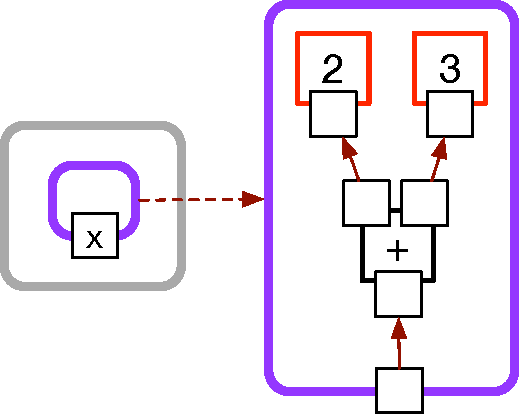
\includegraphics[width=0.5\linewidth]{fig/exp1_gromet_FN_manual_diagram.pdf}
\caption{\gromet\ Function network for exp1.}
\end{figure}


\lstinputlisting[caption=\gromet\ for example exp1., label=exp1]{gromet/exp1--Gromet-FN-auto.json}    

\begin{eqnarray*}
    exp1.fn.x &=& exp1.fn.pof[0]\\
    exp1.fn.pof[0] &=& exp1.fn.bf[0].value.fn.opo[0]\\
    exp1.fn.bf[0].value.fn.opo[0] &=& exp1.fn.bf[0].value.fn.pof[2]\\
    exp1.fn.bf[0].value.fn.pif[0] &=& exp1.fn.bf[0].value.fn.pof[0]\\
    exp1.fn.bf[0].value.fn.pif[1] &=& exp1.fn.bf[0].value.fn.pof[1]\\
    exp1.fn.bf[0].value.fn.pof[2] &=& exp1.fn.bf[0].value.fn.pif[0] + exp1.fn.bf[0].value.fn.pif[1]\\
    exp1.fn.bf[0].value.fn.pof[0] &=& exp1.fn.bf[0].value.fn.bf[0].value\\
    exp1.fn.bf[0].value.fn.bf[0].value &=& 2\\
    exp1.fn.bf[0].value.fn.pof[1] &=& exp1.fn.bf[0].value.fn.bf[1].value\\
    exp1.fn.bf[0].value.fn.bf[1].value &=& 3\\
\end{eqnarray*}

\section{Symbolic Execution Encoding}

\subsection{Examples}

\subsubsection{exp0}
\begin{itemize}
    \item Recurse the expo0 tree to identify the leaf node: $exp0.attr[0].bf[0].value = (2, \phi_0)$, where $2$ is the concrete value and $\phi_0$ is the symbolic value.
    \item Pass the box function value to its output port: $exp0.attr[0].pof[0] = exp0.attr[0].bf[0].value = (2, \phi_0)$.
    \item Pass the output port value to the outer output port: $exp0.attr[0].opo[0] = exp0.attr[0].pof[0] = (2, \phi_0)$
    \item Pass the outer output port to the containing box function output port: $exp0.pof[0] = exp0.attr[0].opo[0] =  (2, \phi_0)$
    \item Associate the name of the output port with the value of the output port: $exp0.x = exp0.pof[0] =  (2, \phi_0)$
\end{itemize}

\subsubsection{Conditional}


\section{Parameter Synthesis}

Let ps(b1, b2, b3) = [([0, 0.5], [0.1, 0.2], [0.8, 0.95]), ([0.51, 0.52], [0.0, 0.09], [0.8, 0.95])]
Let ps(b) = [([0.3, 0.51]), ([0.6, 0.9])]

A parameter space is represented (here) as a list of hypercubes, where a hypercube is a tuple of intervals (one for each dimension).

If I take the project onto b1, I get ps_b2,b3(b1) = [([0, 0.5]), ([0.51, 0.52])]

Intersecting this with ps(b) I get Intersect(ps_b2,b3(b1), ps(b)) = [([0.5, 0.51])]

This is saying that there exists a value of b2 and a value of b3 where for all values of b1 in the intersection (above) the models agree when b1 = b. This is one of many ways of comparing the parameter spaces, but is probably the most simple.

Another way to do it is to define a ps(b') that intersects ps(b1, b2, b3) with a special parameter space ps=(b1, b2, b3) that is defined as the points (degenerate hypercubes) where b1=b2=b3. For example, Intersect(ps(b1, b2, b3), ps=(b1, b2, b3)) = [] because there are no hypercubes in ps(b1, b2, b3) where b1=b2=b3. If we had some ps = [([0.0, 0.3], [0.2, 0.4])], then intersecting it with a similar 2-D parameter space where the parameters are equal would result in a range [0.2, 0.3] (there are infinitely many point hypercubes, so I represent it as a range).

\section{Model Comparison}

Coming soon ... 

\end{document}
